%%%%(c)
%%%%(c)  This file is a portion of the source for the textbook
%%%%(c)
%%%%(c)    Abstract Algebra: Theory and Applications
%%%%(c)    Copyright 1997 by Thomas W. Judson
%%%%(c)
%%%%(c)  See the file COPYING.txt for copying conditions
%%%%(c)
%%%%(c)
\chapter*{Preface}
 
% Print versions need a ToC entry
% tex4ht versions get their own ToC automatically
\ifthenelse{\boolean{basic}\or\boolean{vcu}}{%
\phantomsection
\addcontentsline{toc}{chapter}{Preface}
\pagestyle{myheadings}
\markboth{PREFACE}{PREFACE}
}{}
 
 
 
 
This text is intended for a one- or two-semester undergraduate course
in  abstract algebra. Traditionally, these courses have covered the
theoretical aspects of groups, rings, and fields.  However, with the
development of computing in the last several decades, applications
that involve abstract algebra and discrete mathematics have become
increasingly important, and many science, engineering, and computer 
science students are now electing to minor in mathematics. Though
theory still occupies a central role in the subject of abstract
algebra and no student should go through such a course without a good
notion of what a proof is, the importance of applications such as
coding theory and cryptography has grown significantly.


Until recently most abstract algebra texts included few if any
applications. However, one of the major problems in teaching an
abstract algebra course is that for many students it is their first
encounter with an environment that requires them to do rigorous
proofs. Such students often find it hard to see the use of learning to
prove theorems and propositions; applied examples help the instructor
provide motivation. 
 
 

This text contains more material than can
possibly be covered in a single semester.  Certainly there is adequate
material for a two-semester course, and perhaps more; however, for a
one-semester course it would be quite easy to omit selected chapters
and still have a useful text.  The order of presentation of topics is
standard: groups, then rings, and finally fields. Emphasis can be
placed either on theory or on applications. A typical one-semester
course might cover groups and rings while briefly touching on field
theory, using Chapters~1 through 6, 9, 10, 11, 13 (the first part), 16, 17,
18 (the first part), 20, and 21. Parts of these chapters could be
deleted and applications substituted according to the interests of the
students and the instructor. A two-semester course emphasizing theory
might cover Chapters~1 through 6, 9, 10, 11, 13 through 18, 20, 21, 22 (the
first part), and 23. On the other hand, if applications are to be
emphasized, the course might cover Chapters 1 through 14, and 16
through 22. In an applied course, some of the more theoretical results
could be assumed or omitted. A chapter dependency chart appears below.
(A broken line indicates a partial dependency.)  



\begin{figure}[htb]


\begin{center}

\tikzpreface{dependencies}

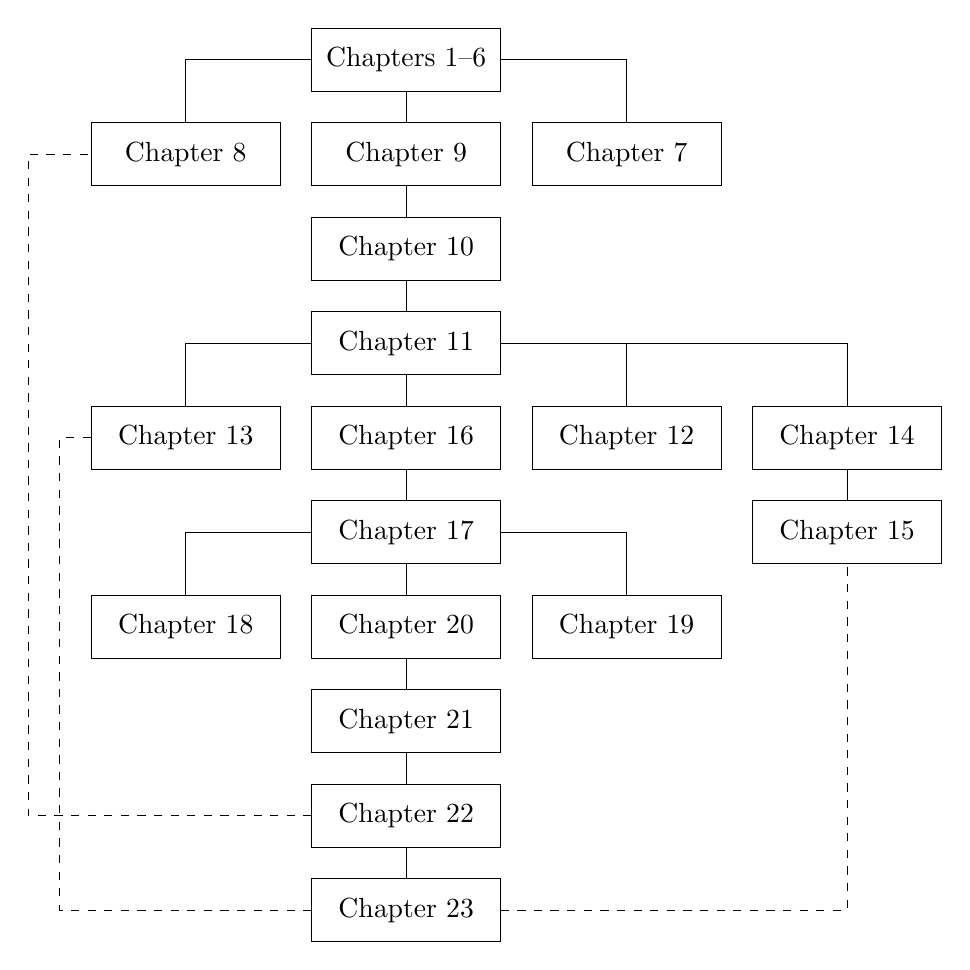
\begin{tikzpicture}[scale=0.8]  %Replaced figure with tikz figure - TWJ 6/14/2010

\draw (3.5,0) rectangle (6.5,1);
\node at (5,0.5) {Chapter 23};

\draw (3.5,1.5) rectangle (6.5,2.5);
\node at (5,2) {Chapter 22};

\draw (3.5,3) rectangle (6.5,4);
\node at (5,3.5) {Chapter 21};

\draw (0,4.5) rectangle (3,5.5);
\node at (1.5,5) {Chapter 18};

\draw (3.5,4.5) rectangle (6.5,5.5);
\node at (5,5) {Chapter 20};

\draw (7,4.5) rectangle (10,5.5);
\node at (8.5,5) {Chapter 19};

\draw (3.5,6) rectangle (6.5,7);
\node at (5,6.5) {Chapter 17};

\draw (10.5,6) rectangle (13.5,7);
\node at (12,6.5) {Chapter 15};

\draw (0,7.5) rectangle (3,8.5);
\node at (1.5,8) {Chapter 13};

\draw (3.5,7.5) rectangle (6.5,8.5);
\node at (5,8) {Chapter 16};

\draw (7,7.5) rectangle (10,8.5);
\node at (8.5,8) {Chapter 12};

\draw (10.5,7.5) rectangle (13.5,8.5);
\node at (12,8) {Chapter 14};

\draw (3.5,9) rectangle (6.5,10);
\node at (5,9.5) {Chapter 11};

\draw (3.5,10.5) rectangle (6.5,11.5);
\node at (5,11) {Chapter 10};

\draw (0,12) rectangle (3,13);
\node at (1.5,12.5) {Chapter 8};

\draw (3.5,12) rectangle (6.5,13);
\node at (5,12.5) {Chapter 9};

\draw (7,12) rectangle (10,13);
\node at (8.5,12.5) {Chapter 7};

\draw (3.5,13.5) rectangle (6.5,14.5);
\node at (5,14) {Chapters 1--6};

\draw (5,1) -- (5,1.5) (5,2.5) -- (5,3)  (5,4) -- (5,4.5)  (5,5.5) -- (5,6)  (5,7) -- (5,7.5)  (5,8.5) -- (5,9)  (5,10) -- (5,10.5)  (5,11.5) -- (5,12)  (5,13) -- (5,13.5);

\draw [dashed] (6.5,0.5) -- (12,0.5) -- (12,6);

\draw (12,7) -- (12,7.5) (12,8.5) -- (12,9.5) -- (6.5,9.5) (8.5,8.5) -- (8.5,9.5);

\draw (8.5,5.5) -- (8.5,6.5) -- (6.5,6.5);

\draw (8.5,13) -- (8.5,14) -- (6.5,14);

\draw [dashed] (3.5,0.5) -- (-0.5,0.5) -- (-0.5,8) -- (0,8);

\draw [dashed] (3.5,2) -- (-1,2) -- (-1,12.5) -- (0,12.5);

\draw (1.5,5.5) -- (1.5,6.5) -- (3.5,6.5);

\draw (1.5,8.5) -- (1.5,9.5) -- (3.5,9.5);

\draw (1.5,13) -- (1.5,14) -- (3.5,14);

\end{tikzpicture}

\end{center}
\end{figure}

Though there are no specific prerequisites for a course in abstract
algebra, students who have had other higher-level courses in
mathematics will generally be more prepared than those who have not,
because they will possess a bit more mathematical sophistication.
Occasionally, we shall assume some basic linear algebra; that is, we
shall take for granted an elementary knowledge of matrices and
determinants. This should present no great problem, since most
students taking a course in abstract algebra have been introduced to
matrices and determinants elsewhere in their career, if they have not
already taken a sophomore- or junior-level course in linear algebra.

Exercise sections are the heart of any mathematics text. An exercise
set appears at the end of each chapter. The nature of the exercises
ranges over several categories; computational,  conceptual, and
theoretical problems are included. A section presenting hints and
solutions to many of the exercises appears at the end of the text.
Often in the solutions a proof is only sketched, and it is up to the
student to provide the details. The exercises range in difficulty from
very easy to very challenging. Many of the more substantial problems
require careful thought, so the student should not be discouraged if
the solution is not forthcoming after a few minutes of work. 
% A complete solutions manual is available for the instructor's use. 
% Removed reference to the solutions manual.  TWJ 8/19/2010

There are additional exercises or computer projects at the ends of
many of the chapters. The computer projects usually require a
knowledge of programming. All of these exercises and projects are more
substantial in nature and allow the exploration of new results and
theory.

% Added Sage blurb, RAB 2011/07/28
Sage (\url{sagemath.org}) is a free, open source, software system
for advanced mathematics, which is ideal for assisting with a study
of abstract algebra. Comprehensive discussion about Sage, and a
selection of relevant exercises, are provided in an electronic
format that may be used with the Sage Notebook in a web browser,
either on your own computer, or at a public server such as
\url{sagenb.org}.  Look for this supplement at the book's
website: \url{abstract.pugetsound.edu}.  In printed
versions of the book, we include a brief description of Sage's
capabilities at the end of each chapter, right after the references.

\section*{Acknowledgements}

I would like to acknowledge the following reviewers for their helpful
comments and suggestions. 
\begin{itemize}
 
\item
David Anderson,
University of Tennessee, Knoxville

\item
Robert Beezer,
University of Puget Sound

\item
Myron Hood,
California Polytechnic State University

\item
Herbert Kasube,
Bradley University

\item
John Kurtzke,
University of Portland
 
\item
Inessa Levi,
University of Louisville
 
\item
Geoffrey Mason,
University of California, Santa Cruz

\item
Bruce Mericle,
Mankato State University
 
\item
Kimmo Rosenthal,
Union College

\item
Mark Teply,
University of Wisconsin

\end{itemize}
I would also like to thank Steve Quigley, Marnie Pommett, Cathie
Griffin, Kelle Karshick, and the rest of the staff at PWS for their
guidance throughout this project. It has been a pleasure to work with
them. 

 
\begin{flushright}
Thomas W. Judson
\end{flushright}
 
 
\pagestyle{headings}
 
 
 
 
